\documentclass{article}
\usepackage{fullpage}
\usepackage{amsmath}
\usepackage{amssymb}
\usepackage{natbib}
\usepackage[linesnumbered,ruled,vlined]{algorithm2e}
\usepackage{algpseudocode}
\usepackage{tikz}
\usetikzlibrary{arrows, snakes,backgrounds}
\tikzstyle{place}=[circle,draw=black,thick, inner sep=0pt, minimum size = 5mm]

\SetKwInput{input}{Input}
\SetKwInput{output}{Output}

\newcommand{\E}{\mathbb{E}}
\renewcommand{\P}{\mathbb{P}}
\newcommand{\R}{\mathbb{R}}


\begin{document}


% Name ideas:
% 
% extend edges
% bundle edges
% inflate edges
% bundle lines of descent
% longer ancestral haplotypes
% inflated ancestors
% compress paths
% optimizing edge tables
% reduce number of ancestors
% reduce ancestral paths

\section{Introduction}

% PETER
% * what's a tree sequence
% * why is a tree sequence (motivation)

The pedigree that describes how everyone of some species
are related to each other
is a large graph, where nodes are indexed by time.
Within this, one can trace back the paths along which segement of genome
have been inherited.
The \emph{succinct tree sequence} (or, tree sequence for short)
was introduced by \citet{kelleher2016efficient} to describe the subset of these paths
along which the genome of a sample of individuals was inherited.


\section{Motivation and statement of problem}

% PETER
% * minimize number of edges
% * gives extra info about shared haplotypes, reduces number of ancestral paths


\section{Algorithm}

% * description (HALLEY)
% * proof of something:
%     - arrives at a local minimum?
%     - guess at typical reduction?

\section{Notation}
    We begin with some notation. We define a \textit{tree sequence}, denoted $TS$ (use Psi), 
    as a tuple $\left( \left\{T_k\right\}, N, E, L\right)$ where
     $\left\{T_k\right\}_{k=1}^n$ is the set of trees,
     $N$ and $E$ are the sets of nodes and edges respectively,
     and $L=[0,a)\subseteq \R$ is the length of the sequence on the genome. 
    Additionally, a node $x\in N$ is \textit{unary} if it only has one child, 
    ie. only a single edge extending below it on the tree.
    With these tree sequences our goal is to
    minimize the number of edges
    as well as infer coalescence of genes. 
    To remove edges we consider the following example.
    Suppose for a tree $T_k$ in the tree sequence $TS$ 
    there exists a branch which contains a unary node $b\in N$.
    Then the node $b$ has one parent, $a\in N$, 
    and one child $c\in N$,
    each with edges $e_{ab}, e_{bc}\in E$ connecting them.
    If there is an edge between the nodes $a$ and $c$ in trees 
    $T_{k+1}$ (or $T_{k-1}$),
    then we wish to extend the edges $e_{ab},e_{bc}$ 
    to $T_{k+1}$ and then remove the edge $e_{ac}$ from $T_{k+1}$. 
    This action reduces the length of the edge $e_{ac}$ on the genome,
    and in some cases, completely removes the edge. 
    We now perform this action on all such unary nodes 
    over the entire tree sequence.

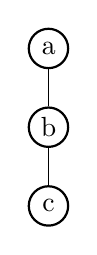
\begin{tikzpicture} %% Do this with phylogenetic trees using tikz (WILL NEED LUALATEX COMPILER) %%
\node[place] (a)  {a};
\node[place] (b)  [below of = a] {b};
\node[place] (c)  [below of = b] {c};
\draw [-] (a.south) -- (b.north);
\draw [-] (b.south) -- (c.north);
\end{tikzpicture}

    In full detail, let $TS = \left( \left\{T_k\right\}_{k=1}^n, N, E, L\right)$
    be a tree sequence.


\begin{algorithm}  % How 'code-like' do we want the algorithm to be? Do we want to keep a lot of the syntax in layman's terms or do we want to use functions like ts1.coiterate(ts2)??
\caption{Extend Edges}\label{alg:cap}
\begin{algorithmic}
\SetKwFunction{mirror}{Mirror Coordinates}
\State   $ N' \gets N$
\State   $ e'\in E' \gets E $
\State   $ T'_k \gets T_{n-k} $
\State   $ T' \gets (\{T'_k\}_{k=1}^n,N',E',L) $ 
\end{algorithmic}
\end{algorithm}

With this algorithm we only extend existing edges
over a larger interval on the genome,
and remove unnecessary edges in the process.
%% Find counter example to global minimum.

\section{Results (how it works)}

% (AVA)
% * reduction in edges ~ sequence length
% * speed increase ~ sequence length
% * proprotion of added edges that are true ~ sequeence length
% * apply to real data:
%     - % fewer edges
%     - % fewer distinct ancestors (ancestral paths?) of sample at some time

\section{Discrepancy Function}
% * How to measure agreement that includes haplotypes
% * Definition and Algorithm
% * Supp fig: runtime ~ # trees, samples
% * fig: how add edges rueduces discrepancy
%       - compare to Relate and tsinfer
% * Show: how add edges reduces discrepancy
% * THINK of a way to asynchronously computing discrepancy

\begin{algorithm}[!ht]


\input{$(x,ts_1,ts_2)$}
\output{discrepancy number (some float value)}

$sim \gets np.zeros(ts2.num_nodes)$\;

\caption{Node Tree Discrepancy}\label{ndisc}
\end{algorithm}

\section{Data}
% * 1. Simulate data
% * 2. Run tsinfer
% * 3. Compare d(x,truth) for x in tsinfer, tsinfer+add edge, tsinfer+add edge + simplify, tsinfer+simplify

% * How much unary edges?
% * How much can we add?

\bibliography{references}

\end{document}
